%% ------------------------------------------------------------------------- %%
\chapter{Conclus�es}
\label{cap:conclusoes}


\section{Descri��o}


Os experimentos consistiram em medir a acur�cia da IFT ao separar objeto e fundo de uma imagem. Os experimentos foram rodados para o banco de imagens p�blicas do grabcut que cont�m 50 imagens. 
Pode-se considerar que foram feitos duas classes de rotinas principais:

\begin{itemize}
\item IFT sobre uma imagem bruta, sem pr�-processamento em regioes (n�vel de pixels).
\item IFT sobre regioes geradas pelo m�todo SLIC, com 100, 400, 900 e 1600 superpixels.
\end{itemize}



\begin{figure}[!h]
\begin{center}
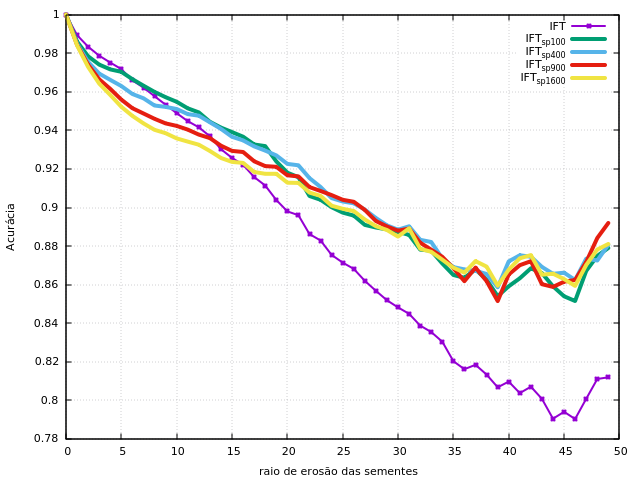
\includegraphics[width=14cm]{figuras/resultados}
\caption{\label{fig:resultados} resultados dos experimentos}
\end{center}
\end{figure}
